\documentclass[a4paper,12pt]{article}
\usepackage[hmargin=2cm,top=4cm,headheight=65pt,footskip=45pt]{geometry}
\usepackage[utf8]{inputenc}
\usepackage{graphicx}
\usepackage[hidelinks]{hyperref}
\usepackage{array}
\usepackage{lastpage}
\usepackage{lipsum}
\usepackage{fancyvrb}
\usepackage{color}
\usepackage{fancyhdr}
\usepackage{amsmath}
\usepackage{enumitem}
\usepackage{titlesec}
\usepackage{floatrow}
\usepackage{float}
\usepackage{subcaption}
\usepackage{caption}
\usepackage{multicol}
\newfloatcommand{capbtabbox}{table}[][\FBwidth]

\definecolor{customGray}{RGB}{128,128,128}
\definecolor{Eblue}{rgb}{0.0, 0.18, 0.39}
%==============Header & Footnote==============

\pagestyle{fancy}
\renewcommand{\headrulewidth}{0pt}
\fancyhead[C,CO,L,LO,R,RO]{}
\fancyhead[C]{%
          \begin{tabular}{|m{3.0cm}|m{10.0cm}|m{2.5cm}|}
          \hline
          \centering\vspace{1.75mm}
\includegraphics[scale=0.275]{logo.pdf} &
          \centering
          {\footnotesize {\sf UNIVERSIDAD EAFIT\\ SCHOOL OF ENGINEERING\\
          \vspace{-1mm}DEPARTMENT OF SYSTEMS AND INFORMATICS}} &
          \centering
          \footnotesize{Page \thepage\ de \pageref{LastPage}\\
          ST245\\
          \vspace{-0.75mm}Data Structures
          }\tabularnewline
          \hline
          \end{tabular}
}
\fancyfoot[C,CO,L,LO,R,RO]{}
\fancyfoot[C]{
          \begin{centering}
            \textcolor{customGray}{{\footnotesize {\sf Professor Mauricio Toro Bermúdez\\
            Phone: $(+57) (4) 261 95 00$ Ext. $9473$. Office: $19 - 627$\\
            \vspace{-1mm}E-mail: mtorobe@eafit.edu.co}}}
        \end{centering}
}

%=============CustomEnumItem===========

\setlist[enumerate]{label=\color{Eblue}\textbf{\roman*.}}

%=============CustomSecSubSec==========

\titleformat{\section}[hang]
{\normalsize\bfseries\itshape\color{black}}{\bfseries\itshape\color{Eblue}\thesection)}{2.5mm}{}

\titleformat{\subsection}[hang]
{\normalsize\bfseries\itshape\color{black}}{\bfseries\color{Eblue}\thesection.\alph{subsection}.}{2.5mm}{}

%==============Title==============

\title{\color{Eblue}\textbf{Laboratory practice No. 5: Binary Trees}}
\author{
  \textbf{Juan S. Cárdenas Rodríguez}\\
  Universidad EAFIT\\
  Medellín, Colombia\\
  jscardenar@eafit.edu.co
\and
  \textbf{David Plazas Escudero}\\
  Universidad EAFIT\\
  Medellín, Colombia\\
  dplazas@eafit.edu.co
}

%=============Document=============
\begin{document}
  \maketitle
  \thispagestyle{fancy}
  \section{Code for delivery on GitHub}
    \subsection{Graphs implementation}
      The code for both implementations is inside the \texttt{DataStructures.py} file in the codigo folder.
    \subsection{Most Children}
      The code can be found inside the \texttt{Code.py} file in the codigo folder.
    \subsection{Test with Dijkstra's alorithm}
      The tests and the implementation for Dijkstra's algorithm can be found inside the \texttt{Code.py} file
      inside the codigo folder.
    \subsection{City-Based Graph}
      The code can be found in the \texttt{City.py} file in the codigo folder.
  \section{Online Exercises}
    The solution to the problem can be found in the \texttt{Code.py} file in the codigo folder.
  \section{Other questions}
    \subsection{Proof for 1.3}
      \begin{figure}[H]
        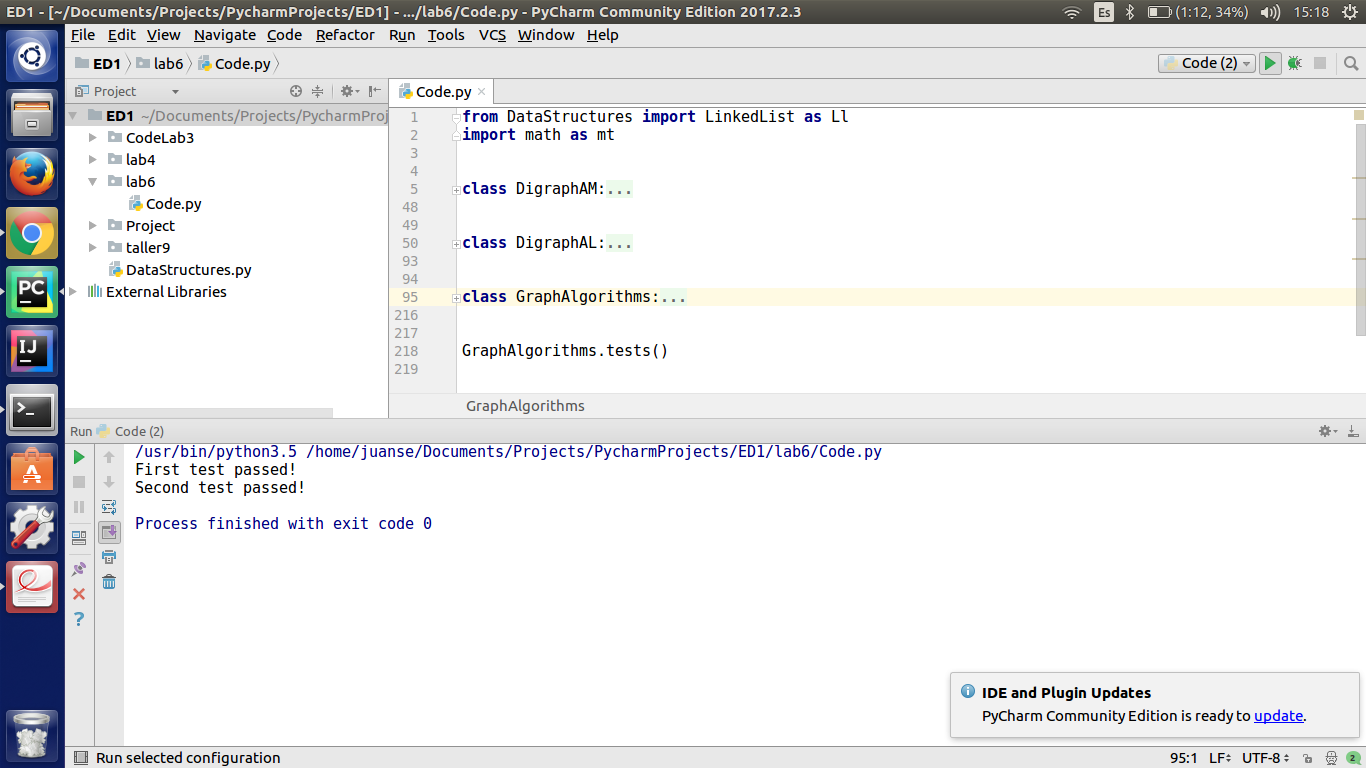
\includegraphics[scale=0.3]{appro.png}
        \caption{Proof for exercise 1.3}
      \end{figure}
    \subsection{Explanation for 1.1}
    Both are digraphs, since the edges have direction. Both have a data structure
    to save the edges' information; the first one has a matrix $A_{nxn}$ that inserts
    a GraphObj in the position $i,j$ if the node $i$ is connected with the $j$ one. The GraphObj
    has value, weight and a Python dictionary for further attributes of the edge. On the
    other hand, the second implementation has a linked list with all the children (nodes that
    are connected to the node we are on). The insertion works similarly in both cases, the user has
    to insert the parent and the child, making an edge between the parent and the child. Check the
    \texttt{DataStructures.py} file in the codigo folder for the source code.

    \subsection{On which graphs is better to use the matrix implementation and on
    which cases is better to use the linked list one?}
    The matrix representation is more useful when the important things are the
    connections, not the weights; so, in a simple graph the matrix representation
    is a fairly good approach to represent it better. But, the priority is to use
    ''greedy algorithms'' or a really big sample of data de linked list
    representation is much better.

    \subsection{Which implementation is better for a city-based graph?}
    As we know that it is a graph related to a city, one can note that it is not possible
    (or HIGHLY unlikely) that all nodes are connected to each other. Therefore, if a matrix
    representation is used, there will be a lot of empty spaces in the matrix. So it is definitely
    better to implement the liked list representation for a city graph.

    \subsection{Which implementation is better for a facebook-based network?}
    It's better to use the linked list representation because, of the big size
    of the data (so we can optimize memory) and this type of data is a priority to
    search for smallest path and more.

    \subsection{Which implementation is better for a routing table?}
    The linked list implementation will be more practical since one will be interested in the
    nodes that are connected; therefore, if this implementation is used, you will know immediately
    the nodes that are connected, you won't have to check the whole row in the matrix for the nodes
    connected. Additionally, the matrix one consumes a lot of memory, which is never good.

    \subsection{Complexity of exercise 2.1}
      \begin{Verbatim}
        @staticmethod
        def bi():
            n = int(input())
            graphs = []
            while n != 0:
                graph = DigraphAM(n)
                graphs.append(graph)
                connections = int(input())
                for i in range(connections):
                    rel = input().split(" ")
                    graph.insert(int(rel[0]), int(rel[1]))
                    graph.insert(int(rel[1]), int(rel[0]))
                n = int(input())

            def bi_color(graph):
                color = [0] * graph.n  # c1
                visit = [False] * graph.n # c2

                def dfs(node, active):  # O(n)
                    children = graph.search(node)
                    color[node] = active
                    visit[node] = True
                    for child in children:
                        if not visit[child]:
                            if active == 1:
                                dfs(child, 0)
                            else:
                                dfs(child, 1)

                dfs(0, 1)  # O(n)

                for i in range(graph.n):  # c3 * n
                    children = graph.search(i)  # Matrix: O(n)
                                                # Linked List: O(m)
                    for child in children:  # c4 * n * m
                        if color[child] == color[i]: # c3 n * m
                            return False

                return True #

            for graph in graphs:
                if bi_color(graph):
                    print("Is bi colorable")
                else:
                    print("Is not bi colorable")

      \end{Verbatim}
      Then, exercise 2.1 is $O(mn)$, where n is the number of vertex and m is the maximum amount of
      children that a vertex has.

    \section{Exam simulation}
      \begin{enumerate}
        \item
          \begin{Verbatim}
            0 1 2 3 4 5 6 7
          0       1 1
          1 1   1     1
          2   1     1   1
          3               1
          4     1
          5
          6     1
          7
          \end{Verbatim}
        \item
          \begin{Verbatim}
            0 -> 3 4
            1 -> 0 2 5
            2 -> 1 4 6
            3 -> 7
            4 -> 2
            5 ->
            6 -> 2
            7 ->
          \end{Verbatim}
        \item
        \begin{table}[H]
        \centering
        \caption{DFS and BFS for each vertex.}
        \begin{tabular}{ccc}
        \hline
        \textbf{Vertex}           & \textbf{DFS} & \textbf{BFS} \\ \hline
        \textbf{0} & 3742156      & 3472165      \\
        \textbf{1} & 0372465      & 0253467      \\
        \textbf{2} & 1037546      & 1460537      \\
        \textbf{3} & 7            & 7            \\
        \textbf{4} & 2103756      & 2160537      \\
        \textbf{5} &              &              \\
        \textbf{6} & 2103754      & 2140537      \\
        \textbf{7} &              &              \\ \hline
        \end{tabular}
        \end{table}
        \item a) $O(n)$
        \item
          \begin{Verbatim}
            def aPath(graph,p,q):
              seen = [False]*graph.size
              return aPathAux(graph,p,q,[],seen)

            def aPathAux(graph,p,q,myList,seen):
              if p == q:
                if len(myList) == 0:
                  myList.append(q)
                return myList

              children = graph.getSuccesors(p)
              for child in children:
                if not seen[child]:
                  seen[child] = True
                  myList.append(child)
                  return aPathAux(graph,child,q,myList,seen)
              return
          \end{Verbatim}
      \end{enumerate}







\end{document}
